\chapter{Multi-Modal Interaction-Aware Trajectory Optimisation}
\label{text:approach}
In this chapter an overview of the approach is provided. Starting in section \ref{text:approach/formulation} the problem of socially-aware motion planning is formulated formally, including the assumptions made within this project. 
\newline
Section \ref{text:approach/overview} which presents an overview over the full trajectory optimisation pipeline. It is shown how the algorithm is built in order to allow to deal with general graph-like pedestrian behaviour prediction models, with multi-modal, probabilistic outputs. Furthermore, the advantages of formulating socially-aware motion planning as an optimisation problem while utilising graph-based prediction model, e.g. deep learning based models such as the Trajectron \cite{Ivanovic18}, over purely learned \cite{Chen2017} or purely optimisation-based \cite{Berg2011} algorithms are illustrated. Finally it is explained how the usage of a general-purpose, computation-graph based framework such as PyTorch \cite{pytorch} or TensorFlow \cite{tensorflow} can be harnessed for a highly modular, efficient and versatile implementation.
\newline
The exact formulation of the optimisation problem is further explained in section \ref{text:approach/objective} and \ref{text:approach/constraint}. Beginning with the objective function the both the goal-driven and the interaction-driven parts are illustrated, together with a derivation of their gradients. Furthermore, several designs of the specific objective function are discussed. The subsequent section addresses the design of the constraints used. Likewise several constraint function designs are compared. 
\newline
In order to use the system in real-world applications it must comply several requirements. While some of these has been tackled by the optimisation design, e.g. feasibility of the control limitations of the robot or safety regarding robot-human interaction, the system underlies runtime limits. Similarly to \cite{Chen2017} this project aims to run at a frequency of $10 Hz$. To achieve this goal several runtime improvements have been implemented, which are described in section \ref{text:approach/runtime}.


\section{Problem Formulation}
\label{text:approach/formulation}
In this work we are interested in finding the optimal trajectory for a robot navigating among pedestrians on the two-dimensional plane. Let $\x_t = (x_t, y_t, \dot{x}_t, \dot{y}_t) \in \mathbb{R}^4 $ be the position and velocity of the robot, also referred as $ego$, at time $t$ and $\x_{0:N}$ a trajectory over multiple states $(\x_0, \x_1, \x_2, \hdots, \x_N)$. Within this work the robot is assumed to have double integrator dynamics. With control input $\u_t = (u_{x, t}, u_{y, t}) \in \mathbb{R}^2$ and system dynamics $f(\cdot)$, we have: 

\begin{align}
\ddot{\x}_t &= \u_t \\
\dot{\x}_t &= f(\x_t, \u_t)
\label{eq:robot_dynamics}
\end{align}

For further simplification the robot's dynamics are assumed to be deterministic.
\newline
In general each pedestrian's trajectory is probabilistic and multimodal. Thereby,  let $\xped[k]_t = \mathbf{\tilde{\xi}_t^k}$ be the state distribution of pedestrian $k$ at time $t$, with mean $\mathbf{\tilde{\mu}_t^k}$, variance $\mathbf{\tilde{\Sigma}_t^k}$ and mode-weights vector $\mathbf{\tilde{\pi}_t^k}$. 

\begin{equation}
\xped[k]_t \sim \mathbf{\tilde{\xi}_t^k}(\mathbf{\tilde{\mu}_t^k}, \mathbf{\tilde{\Sigma}_t^k}, \mathbf{\tilde{\pi}_t^k})	
\end{equation}

Similar to the robot the pedestrians are modelled as single point masses. The pedestrian's trajectories are predicted using some model $\tilde{\Phi}$ which is assumed to be known. As described above in general for some pedestrian $k$ the model $\tilde{\Phi}_k$ outputs a multi-modal distribution over the next state $\xped[k]_{t+1}$ conditioned on the trajectory of the robot $\x_{0:t}$, the trajectory of every other pedestrian in the scene $\xped[j]_{0:t} (j \neq k)$ and the trajectory of the pedestrian $k$ itself, i.e. $\xped[k]_{0:t}$. Moreover the function $\tilde{\Phi}$ is generally not shared over all pedestrian, but individually for each one.

\begin{equation}
\xped[k]_{t+1} = \tilde{\Phi}_k(\x_{0:t}, \xped[i]_{0:t}) \quad \forall i \in [0, K]	
\end{equation}

Furthermore both the robot and the pedestrians underly constraints for their minimal and maximal control effort. Thus, the sets of feasible control inputs $\mathcal{U}$ and $\mathcal{\tilde{U}}$ respectively, are defined as 

\begin{align}
\mathcal{U} &= \{\u | \u \in \mathbb{R}^2, u_{min} \leq ||\u||_2 \leq u_{max}\} \\
\mathcal{\tilde{U}} &= \{\uped[] | \uped[] \in \mathbb{R}^2, \tilde{u}_{min} \leq ||\uped[]||_2 \leq \tilde{u}_{max}\} 
\end{align}
 
Within project \project I want to find a robot trajectory $\x_{0:T}$ over some discrete time horizon $N$ that trade-offs between minimising the travel time from the its current state to some goal state in $\mathcal{X}_f = \{\mathbf{g} | \mathbf{g} \in \mathcal{X} \}$ on the one side and the interference with the pedestrians in the scene on the other side, with respect to its dynamic as well as safety boundaries. For further simplification a perfect knowledge about the current and all past states of surrounding agents $\xped[k]_{0:t} \forall k \in [0, K]$ is assumed. 

\section{System Overview}
\label{text:approach/overview}
The goal of project \project is to develop a trajectory optimisation formulation that strikes a balance between decreasing the cost for reaching some terminal set $\mathcal{X}_f$ and the disturbance on the human behaviour, which the robot introduces by moving among them, and ensuring safety in these interactions. As shown in Figure \ref{img:information_flow} the problem can be divided into several subproblems, which also can be seen as modules of a trajectory optimisation problem and therefore can be formulated independently from each other. 

\begin{figure}[!ht]
\begin{center}

\includegraphics[width=\imgwidth]{images/placeholder.png}
\captionof{figure}{Information-Flow-Diagram}
\label{img:information_flow}
\end{center}
\end{figure}

Formally, the solution to this problem can be represented as the following optimisation problem (comp. Problem \ref{eq:formulation}). In this work the initial time $t_0 = 0$ and the final time $t_f = T \cdot \Delta t$ is used for simple notation, although not required in general \cite{Wachter2006}. \\

\begin{problem} General \project optimisation problem
\begin{equation}
\min_{\u_{0:T-1}} \quad w_{goal} J_{goal}(\x_{0:T}) + w_{int} \sum_{k=0}^M \mathbb{E}_{\xped[k]_{0:T}}[J_{int}(\x_{0:T}, \xped[j]_{0:T})]
\end{equation}
\begin{align}
\textrm{s.t. } \quad & \x_{t+1} = f(\x_t, \u_t) & \forall t \in [0, N] \\
& \xped[k] = \tilde{\Phi}_k(\x_{0:t}, \xped[i]_{0:t}) & \forall k \in [0, K], \forall t \in [0, N]\\
& g_{safety}(\x_{0:T}, \xped[k]_{0:T}) \leq 0 & \forall k \in [0, K] \\
& \x \in \mathcal{X} & \forall t \in [0, N]\\
& \u_t \in \mathcal{U} & \forall t \in [0, N]\\
& \x_0 \in \mathcal{X}_0 \\
& \x_N \in \mathcal{X}_f
\end{align} 
\label{eq:formulation}
\end{problem}

Hence, the objective function is a weighted sum of a goad-driven $J_{goal}(\cdot)$ and some interaction-driven term $J_{int}(\cdot)$, which are further explained in section \ref{text:approach/objective}. The constraints are a combination of dynamics constraints, safety constraints as well as initial and final state restrictions, which are discussed in section \ref{text:approach/constraint}.

% todo: nonzero in equality \& inequality Jacobian, Hessian, number of variables, number of constraints 

\subsubsection{Transcription Method} 
Trajectory optimisation is a wide field with many different methodologies. Though the area can be roughly broken down into two categories, shooting and collocation \cite{Kelly2017}.\footnote{There are several other directions of separation possible such as the direct vs indirect methods, but I will focus on shooting vs collocation here. Further information about the taxonomy of trajectory optimisation can be found in \cite{Kelly2017} and \cite{Chai2020}.} Shooting optimises for the control inputs and unrolls them using a simulation environment to compute objective objective and constraint. Thereby the dynamics constraint $x = f(x, u)$ is intrinsically enforced. In comparison collocation uses all controls and (!) states as decision variables, while constraining the system dynamics, and tries to solve the \ac{NLP} by approximating some function (e.g. Lagrange polynomials in orthogonal collocation). Due to the linear and cheap to compute dynamics, the availability of a simulation engine tightly bound to the optimisation and since the constraints acting on both the path $\x_{0:T}$ itself and the controls $\u_{0:T}$ are comparably "simple", as illustrated in section \ref{text:approach/constraint}, shooting is used within this project. Therefore the trajectory is split up into several segments, one for each discrete discretisation time step, which makes solving problem \ref{eq:formulation} more easier to be solved and more robust (multiple shooting) \cite{Betts1998}.

\subsubsection{Nonlinear Optimisation Solver} 
Since no further assumptions about the pedestrian trajectory prediction model $\tilde{\Phi}$ have been made, the optimisation is non-linear and especially non-convex in general. As shown in \cite{Gould2003}\cite{Parkinson2018}\cite{Freund2004} there are a bunch of algorithms to deal with general non-linear optimisation problems, such as line-search, trust-region, interior-point, generalised-reduced-gradient or sequential-quadratic-programming methods as well as combinations of these such as LOQO. However not all of them are applicable to constrained problems such as Problem \ref{eq:formulation}. For constrained optimisation problems \ac{SQP} and \ac{IPM} are the most popular ones, both having its advantages and drawbacks. While \ac{SQP} usually require less solver iterations and thus less function calls, they scale poorly with the number of constraints and do not guarantee that intermediate results are feasible \cite{Dehdari2013}\cite{Parkinson2018}. Although this can be an advantage in case of computationally expensive constraints, it also leads to an infeasible solution when the algorithm is stopped for convergence. Additionally, compared to \ac{IPM} the computational time required by the solver itself is usually larger (e.g. as demonstrated in \cite{Dehdari2013}).
\newline
In project \project safety is induced by constraint, thus obtaining a feasible solution is crucial, also if the algorithm might be aborted before convergence due to runtime constraints. For this reason an interior-point method has been used within the project. The interior-point method \ac{IPOPT} \cite{Wachter2006} has shown to be applicable in many robotics applications, and has shown to be valuable even in case of very tough runtime constraints such as solving the feedforward commands in high-performance automated driving at 50 Hz in \cite{Spielberge2019} or motion planning for legged robotics \cite{Winkler2018}. There it has been used in this project as well.\footnote{From today's point of view it turned out, after tweaking the performance of the optimisation core as best as possible, it turns out that in fact the number of objective function calls is the bottleneck of the algorithm. Therefore comparing the capacity of interior-point solver such as \ac{IPOPT} with \ac{SQP} solvers such as \ac{GuSTO} remains for future work.} 

\subsubsection{Implementation Details} 
The algorithm has been implemented in Python 3.7 using PyTorch \cite{pytorch}. Next to executing computations highly efficiently by vectorisation and batching PyTorch's automatic differentiation framework allows to compute gradients at low computational cost as well as modular, i.e. without the need to explicitly define its closed form. This is the core of prediction-based optimisation, enabling to define objectives and constraints (such as $J_{int}$), which depend on a complex graph-based computation, and still being able to derive their gradient without  costly and inaccurate numerical approximations.
\newline
The system's integrity has been verified by roughly 1000 unit- and integration tests, secured over the code development by the continuous integration framework CircleCI\footnote{Automated testing framework: https://circleci.com} and CodeCov\footnote{Testing coverage reports: https://codecov.io}.

\section{Objective Function Design}
\label{text:approach/objective}

\subsection{Goal Objective}
\label{text:approach/objective/goal}
The goal objective gives an incentive for the optimiser to choose a solution that targets the goal state. It simply consists of the squared L2-norm between each robot trajectory point and the goal state $\mathbf{g}$, normalised over the full planning horizon $N$:

\begin{equation}
J_{goal}(\x_{0:T}) = \frac{1}{N} \sum_{t = 0}^N (\x_t - \mathbf{g})^2
\end{equation}

By normalisation the cost is independent from the length of the planning horizon and thus allows to use the same weight $w_{goal}$ for different planning horizons (comp. equation \ref{eq:formulation}). In Figure \ref{img:goal_norm_vs_sum} the convergence of both formulations is compared; although the terminal cost is the same, the normalised version (\textit{goal\_norm}) converges slightly faster, presumably due to the smaller starting value. Although shown for only one scenario here, both, the ease in tuning and slightly larger convergence speed of the normalised goal objective can be observed also over a wide variety of different scenarios.  

\begin{figure}[!ht]
\begin{center}
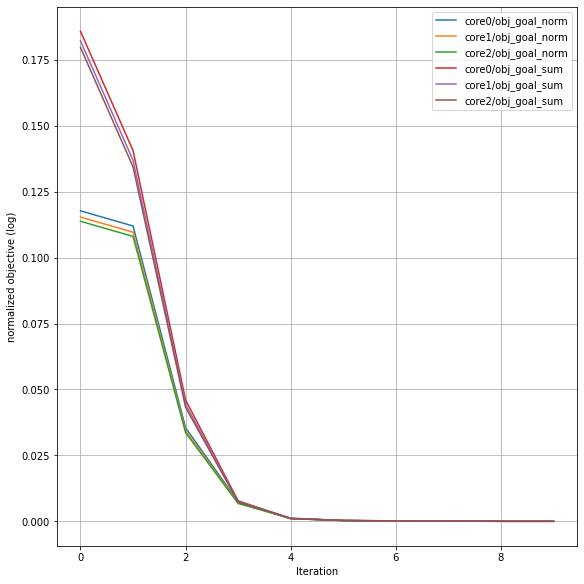
\includegraphics[width=\imgwidth]{images/goal_norm_vs_sum.png}
\captionof{figure}{Direct comparison of a norm-based vs a weighted-sum based goal objective function, normalised by their end value. While roughly the same final objective value is reached (not shown here), the normed goal objective converges faster, i.e. gets to its minimum with fewer iterations over all initial conditions (\textit{core0, core1, core2}). For further details please have a look into the example notebook: \href{https://github.com/simon-schaefer/mantrap/blob/master/examples/modules/goal.ipynb}{examples/modules/goal}.}.
\label{img:goal_norm_vs_sum}
\end{center}
\end{figure}

Since the goal objective $J_{goal}(\x_{0:T})$ is only a function of the robot's planned trajectory and the goal state, its jacobian can be derived without further knowledge of the pedestrian prediction model, merely using the (known) robot dynamics. As described in section \ref{text:approach/overview} the robot controls are optimised. Hence by applying the chain rule we get: 

\begin{equation}
\nabla J_{goal} = \pd{J_{goal}}{\u_{0:T-1}} = \pd{J_{goal}}{\x_{0:T}} \cdot \pd{\x_{0:T}}{\u_{0:T-1}}
\end{equation}

As demonstrated, the goal-objectives gradient can be derived by multiplying the objectives gradient with respect to the robot's trajectory with the gradient of the robot's trajectory with respect to its control inputs. Since the goal-objective directly depends on the trajectory, deriving the first term is straight-forward to derive. The second term $\delta \x_{0:T} / \delta \u_{0:T-1}$ is not trivial in general, because of the iterative structure of rolling out state trajectories based on dynamics and as the robot's dynamics $f(\cdot)$ can be arbitrary, however as described in section \ref{text:approach/formulation} double integrator dynamics are assumed for the robot, so that the whole trajectory $\x_{0:T}$ can be expressed as function of the initial state $\x_0$ and the control inputs $\u_{0:T-1}$ only, as shown in equation \ref{eq:dynamics_stacked}. Then the term $\delta \x_{0:T} / \delta \u_{0:T-1}$ simplifies to a constant term:

\begin{align}
\pd{J_{goal}}{\x_{0:T}} &= \pd{}{\x_{0:T}} \frac{1}{N} \sum_{t = 0}^N (\x_t - \mathbf{g})^2 \\
&= \frac{2}{T} \begin{bmatrix} (\x_1 - \mathbf{g}) & \hdots & (\x_T - \mathbf{g}) \end{bmatrix}^T
\end{align}

\begin{align}
\pd{\x_{0:T}}{\u_{0:T-1}} &= \pd{}{\u_{0:T-1}} \begin{bmatrix} A \x_0 \\ A_n \x_0 + B_n \u_{0:T-1} \end{bmatrix} \\
&= \begin{bmatrix} \mathbf{0}_{n \times m} \\ B_n \end{bmatrix}
\end{align}

with $A_n, B_n$ the stacked state-space description matrices as described in section \ref{text:approach/runtime/unrolling}. 
\newline
Overall the goal objective and its gradient are very efficient, cheap to compute, having linear complexity with the length of the planning horizon $T$ and being independent from the number of pedestrians. Furthermore it is strictly convex, which improves the optimisation convergence speed. Therefore it is quite valuable for warm-starting the optimisation algorithm, as further explained in section \ref{text:approach/runtime/warm_starting}.


%todo: final speed objective

\subsection{Interaction Objective}
\label{text:approach/objective/interactive}

%The prediction $\tilde{\Phi}^k$ of the trajectory of pedestrian $k$ over the planning horizon might be non-linear, multi-modal and probabilistic in general, for example the multi-modal predictions made by the Trajectron in Figure \ref{img:trajectron_example}. With $K$ pedestrians, a prediction of $L$ possible modes per pedestrian, each mode being assigned to some probability distribution $\tilde{\phi}^{k,l}$ 

\section{Constraint Function Design}
\label{text:approach/constraint}

\subsection{Dynamics Constraints}
\label{text:approach/constraint/dynamics}


\subsection{Reachability Constraint}
\label{text:approach/constraint/reachability}

% however they follow single integrator dynamics. As pointed out in \cite{Ivanovic18} this is an intuitive choice "as a person’s movements are all position-changing, e.g. walking increases position along a direction, running does so faster". Other standard models for pedestrian dynamics such as Social Forces \cite{Helbling1995} however regard the pedestrian to be a double integrator, not a single integrator, and describe the forces acting on it introduced by other pedestrians, obstacles, etc. Having a reasonable fast reaction time and a large maximal acceleration in comparison to the robot both of these descriptions converge, so that the single integrator model is a good choice nonetheless.\footnote{As discussed in chapter \ref{text:experiments} the modular implementation allows to use different pedestrian dynamics. When testing against other prediction environments, in fact, non single integrator dynamics are used, but most analysis described in this report relates to the single integrator model.} 

% todo: constraint formulation (e.g. min-distance constraints split to be more accurate or summed to compute jacobian faster)
% todo: Quellen: neural network representation of value function to make it differentiable (Karen: reachability, Kyle David Julian: network representation to make sure all the corner cases are met)

\section{Runtime Optimisation}
\label{text:approach/runtime}

\subsection{Efficient Trajectory Unrolling}
\label{text:approach/runtime/unrolling}
One of the most promising directions for decreasing the runtime of a trajectory optimisation algorithm is to decrease the runtime of the objective and constraints evaluation as well as their gradients. As shown in sections \ref{text:approach/objective} and \ref{text:approach/constraint} the majority of these optimisation modules depends on the robot's trajectory $X_R$, rather than on its control inputs $U_R$. However since control inputs are optimised, as described in section \ref{text:approach/overview}, a computationally efficient transformation from controls and initial state to the trajectory is key for making the trajectory optimisation real-time feasible.
\newline
Fortunately, we assumed that the robot follows double integrator dynamics, which are linear and markovian. Hence, they can be expressed as the following: 

\begin{equation}
\x_{t+1} = A \x_t + B \u_t
\label{eq:dynamics}
\end{equation}

\begin{minipage}{0.5\textwidth}
$$A = \begin{bmatrix} 1 & 0 & \delta t & 0 \\ 0 & 1 & 0 & \delta t \\ 0 & 0 & 1 & 0 \\ 0 & 0 & 0 & 1\end{bmatrix}$$
\end{minipage}
\begin{minipage}{0.5\textwidth}
$$B = \begin{bmatrix} 0 & 0 & \delta t & 0 \\ 0 & 0 & 0 & \delta t \end{bmatrix}$$
\end{minipage}

Due to the linear (not linearised !) dynamics $\delta t = \Delta t$ can be safely used. In order to fully "unroll" a trajectory the linear dynamic equation \ref{eq:dynamics} would be to be applied iteratively for the length of the trajectory. Since the dynamics themselves are linear (not just a first-order approximation) this computation can be further batched and on this way, speeded up. In fact the full trajectory can be derived merely based on the initial state $\x_0$ and the control input matrix $\u_{0:T}$, as shown in the following:

\begin{align}
\x_1 &= A \x_0 + B \ u_0 \\
\x_2 &= A \x_0 + B \ u_1 = A^2 \x_0 + A B \ u_0 + B \ u_1\\ 
\hdots &= \hdots \\
\begin{bmatrix} \x_1 \\ \x_2 \\ \vdots \\ \x_n \end{bmatrix} &= \underbrace{\begin{bmatrix} A \\ A^2 \\ \vdots \\ A^n \end{bmatrix}}_{\substack{A_n}} \x_0 + \underbrace{\begin{bmatrix} B & 0 & \hdots & \hdots & 0 \\ AB & B & 0 & \hdots & 0 \\ \hdots & \hdots & \hdots & \hdots & \hdots \\ A^{n-1} B & A^{n-2} B & \hdots & \hdots & B \end{bmatrix}}_{\substack{B_n}} \begin{bmatrix} \u_0 \\ \u_1 \\ \vdots \\ \u_{n-1} \end{bmatrix}
\end{align}

In summary we get the following (also linear) expression for computing the full robot trajectory at once. As demonstrated in \href{https://github.com/simon-schaefer/mantrap/blob/master/examples/tools/timing.ipynb}{examples/tools/timing} using the fully batched formulation speeds up the trajectory "unrolling" by about a factor of 30.  

\begin{equation}
\x_{1:n} = A_n \x_0 + B_n \u_{0:T-1}
\label{eq:dynamics_stacked}
\end{equation}

\subsection{Warm Starting}
\label{text:approach/runtime/warm_starting}
It is widely known that warm starting an optimisation can be very beneficial for its convergence speed for several optimisation algorithms, e.g. shown in \cite{Banerjee2020} for \ac{GuSTO} or for \ac{IPOPT} in \cite{Shahzad2010}, \cite{John2008} or \cite{Spielberge2019}.
\newline
Within project \project the algorithm has been warm-started by solving the optimisation problem posed in problem \ref{eq:formulation} while ignoring all objectives and constraints that relate to pedestrians, i.e. by solving the following optimisation problem: \\

\begin{problem}{Simplified \project optimisation problem for warm-starting}
\begin{align}
\min_{\u_{0:T-1}} \quad & J_{goal}(\x_{0:T}) \\
\textrm{s.t. } \quad & \x_{t+1} = f(\x_t, \u_t) & \forall t \in [0, N] \\
& \x \in \mathcal{X} & \forall t \in [0, N]\\
& \u_t \in \mathcal{U} & \forall t \in [0, N]\\
& \x_0 \in \mathcal{X}_0 \\
& \x_N \in \mathcal{X}_f
\end{align} 
\label{eq:formulation_warm_starting}
\end{problem}

Since the simplified optimisation problem in problem \ref{eq:formulation_warm_starting} does not depend on the pedestrian dynamics model $\tilde{\Phi}$ it is much easier and more efficient to solve, being a convex quadratic program.

%todo: pre-computation warm-starting since going straight is often not a good choice

\subsection{Attention}
\label{text:approach/runtime/filtering}
